\documentclass[a4paper,twoside]{article} %twoside=dois lados
\usepackage{fontspec}
\defaultfontfeatures{Ligatures={TeX}}
\setmainfont{Minion Pro}
\setsansfont{Myriad Pro}
\setmonofont[Scale=.9]{Consolas}
\usepackage{polyglossia}
\setmainlanguage{brazil}
\setotherlanguages{french,english,german,russian,greek,spanish,italian,norsk}
\usepackage{graphicx}
\usepackage{enumerate}
\usepackage[bookmarks]{hyperref}
\usepackage[dvipsnames]{xcolor}
\usepackage[xcolor]{mdframed}
\usepackage{lipsum}

\title{Título}
\author{Autor}
\date{Data}

%retire se não quiser cabeçalhos===============
\usepackage{fancyhdr}
%\renewcommand{\chaptermark}[1]{\markboth{#1}{}}
\renewcommand{\sectionmark}[1]{\markright{#1}}
\pagestyle{fancy}
\fancyhf{}
\fancyfoot[LE,RO]{\thepage}
\fancyhead[LO]{\itshape\nouppercase{\rightmark}}
\fancyhead[RE]{\itshape\nouppercase{\leftmark}}
\renewcommand{\headrulewidth}{0pt} 
%retire se não quiser cabeçalhos================

\begin{document}

\frenchspacing

\maketitle

\begin{abstract}
Escreva aqui o seu resumo. Escreva aqui o seu resumo. Escreva aqui o seu resumo. Escreva aqui o seu resumo. Escreva aqui o seu resumo. Escreva aqui o seu resumo.
\end{abstract}

\tableofcontents % comente ( % na frente) se não quiser sumário
\listoffigures % comente ( % na frente) se não houver figuras
%\listoftables % descomente (retire o %)se quiser lista de tabelas

%Use \% para porcento; \& para &. Dê espaço de uma linha entre dois parágrafos.
%Use \emph{texto} para itálico.
%Seja feliz.

\section{Coloque o título da seção}
\lipsum[1-5]


\begin{figure}
\centering
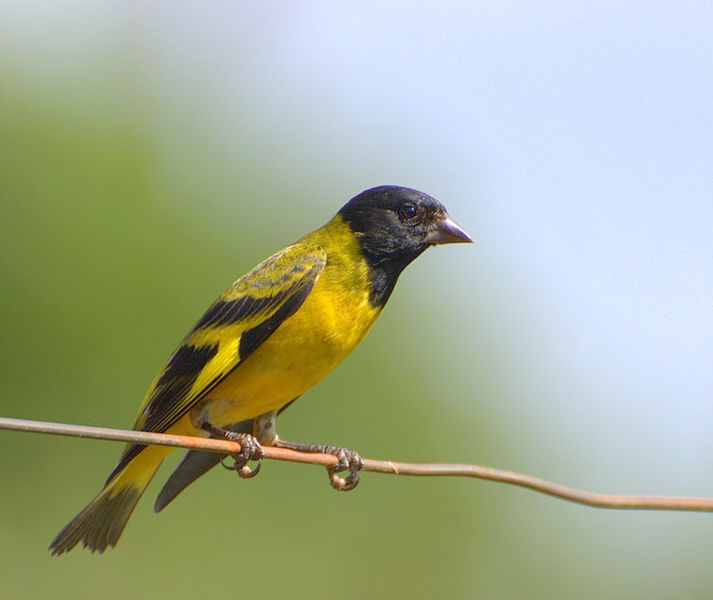
\includegraphics[width=0.5\linewidth]{pintassilgo}
\caption{Pintassilgo-de-cabeça-preta. \textit{Carduelis magellanica}.}
\label{pintassilgo}
\end{figure}



\section{Coloque o título da seção}
\lipsum[1]

\subsection{Subseção}

\lipsum[1-5] %só para preencher com texto sem sentido.



\section{Coloque o título da seção}
\lipsum[1-5]

\section*{Bibliografia}
\addcontentsline{toc}{section}{Bibliografia}

\setlength{\parindent}{0pt}

Schimmel, Annemarie, and Stuart Cary Welch. \textit{Anvari's Divan: A Pocket Book for Akbar}.  New York: The Metropolitan Museum of Art, 1983.

\setlength{\parskip}{10pt} %acrescente depois da primeira entrada bibliográfica

Mearsheimer, John. \textit{The Tragedy of Great Power Politics.} New York and London: W.W. Norton \& Company, 2001.




\end{document}
